

%%%%%%%%%%%%%%%%%%%%%%%%%%%%%%%%%%%%%%%%%%%%%%%%%%%%%%%%%%%%%%%%%%%%%%%%%%%%%
%%%%%%%%%%%%%%%%%%%%%%%%%%%%%%%%%%%%%%%%%%%%%%%%%%%%%%%%%%%%%%%%%%%%%%%%%%%%%
\section{3D parametric linear spline }
A 3D parametric linear spline is a parametric function defined piecewise by parametric polynomials in $\mathbb{R}^{3}$ space.
The Fig. \ref{fig:3DLinearSplinePoly} shows the polynomials $\mathbf{\hat{p}}^{(n)}(t)$ with parameter $t$ 
close to the n-th position.
\begin{figure}[H]
    \centering
    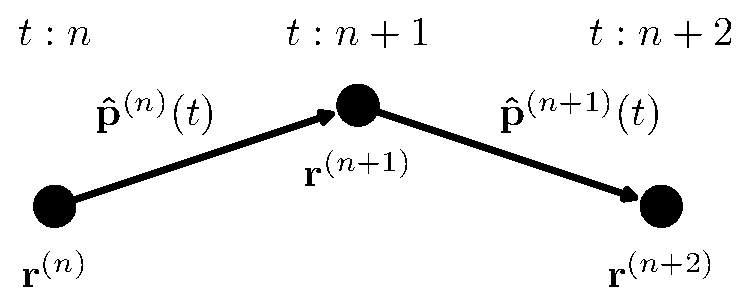
\includegraphics[width=0.35\textwidth]{boveda/Diagrama0.eps}
    \caption{Polynomials in the n-th position of linear spline}
    \label{fig:3DLinearSplinePoly}
\end{figure}

Given a set of $N$ points $\mathbf{r}^{(n)}\in\mathbb{R}^{3}$, $\forall$ $0\leq n \leq N-1$, 
we can generate a linear spline with $N-2$ polynomials $\mathbf{\hat{p}}^{(n)}(t)$, $\forall$ $0\leq n \leq N-2$, 
according to Fig. \ref{fig:3DLinearSplinePoly}.
So that, it is fulfilled that 

\begin{equation}
\mathbf{\hat{p}}^{(n)}(t)=
\begin{bmatrix}
\hat{x}^{(n)}(t) & \hat{y}^{(n)}(t) & \hat{z}^{(n)}(t),
\end{bmatrix}^{T}
\end{equation}
where
\begin{equation}
\hat{x}^{(n)}(t)=\hat{a}_{x}^{(n)}+\hat{b}_{x}^{(n)}(t-n),
\end{equation}
\begin{equation}
\hat{y}^{(n)}(t)=\hat{a}_{y}^{(n)}+\hat{b}_{y}^{(n)}(t-n),
\end{equation}
\begin{equation}
\hat{z}^{(n)}(t)=\hat{a}_{z}^{(n)}+\hat{b}_{z}^{(n)}(t-n).
\end{equation}



%%%%%%%%%%%%%%%%%%%%%%%%%%%%%%%%%%%%%%%%%%%%%%%%%%%%%%%%%%%%%%%%%%%%%%%%%%%%%
\subsection{Matricial form of polynomials $\mathbf{\hat{p}}^{(n)}(t)$}
For all values $0\leq n \leq N-2$, we know that
\begin{equation}
\mathbf{\hat{w}}^{(n)}=
\left[
\begin{array}{cc:cc:cc}
\hat{a}_{x}^{(n)} & \hat{b}_{x}^{(n)} & 
\hat{a}_{y}^{(n)} & \hat{b}_{y}^{(n)} & 
\hat{a}_{z}^{(n)} & \hat{b}_{z}^{(n)} 
\end{array}
\right]^{T},
\end{equation}
\small
\begin{equation}\label{eq:hatAnt}
\mathbf{\hat{A}}^{(n)}(t)=
\left[
\begin{array}{cc:cc:cc}
1 & (t-n) &
0 & 0     &
0 & 0     \\
0 & 0     &
1 & (t-n) &
0 & 0     \\
0 & 0     &
0 & 0     &
1 & (t-n) 
\end{array}
\right],
\end{equation}
\normalsize

\begin{equation}\label{eq:hatprimeder0}
\mathbf{\hat{p}}^{(n)}(t)=
\mathbf{\hat{A}}^{(n)}(t) \mathbf{\hat{w}}^{(n)}.
\end{equation}

Additionally, we can define

\begin{equation}
\mathbf{\hat{w}}
\equiv
\begin{bmatrix}
\mathbf{\hat{w}}^{(0)}\\
\mathbf{\hat{w}}^{(1)}\\
%\mathbf{\hat{w}}^{(2)}\\
\vdots\\
\mathbf{\hat{w}}^{(N-2)}\\
\end{bmatrix}
\in \mathbb{R}^{6(N-1)}
\end{equation}


%%%%%%%%%%%%%%%%%%%%%%%%%%%%%%%%%%%%%%%%%%%%%%%%%%%%%%%%%%%%%%%%%%%%%%%%%%%%%
%%%%%%%%%%%%%%%%%%%%%%%%%%%%%%%%%%%%%%%%%%%%%%%%%%%%%%%%%%%%%%%%%%%%%%%%%%%%%
\subsection{Boundary conditions in 3D parametric linear spline}\label{sec:boundarylinear}

%%%%%%%%%%%%%%%%%%%%%%%%%%%%%%%%%%%%%%%%%%%%%%%%%%%%%%%%%%%%%%%%%%%%%%%%%%%%%
\subsubsection{Conditions in points}

Following the Fig. \ref{fig:3DLinearSplinePoly}, 
we can affirm that for $0 \leq n\leq N-2$,
so that
\begin{equation}\label{eq:hatcondition1}
\mathbf{\hat{p}}^{(n)}(n)=\mathbf{r}^{(n)}
\in \mathbb{R}^{3},
\end{equation}

\begin{equation}\label{eq:hatcondition2}
\mathbf{\hat{p}}^{(N-2)}(N-1)=\mathbf{r}^{(N-1)}
\in \mathbb{R}^{3},
\end{equation}

\textbf{Matricial form of the conditions in points:}

Using 
the Eq. \ref{eq:hatprimeder0} in 
the Eqs. \ref{eq:hatcondition1} and \ref{eq:hatcondition2},
we obtain for $0 \leq n\leq N-2$

\begin{equation}\label{eq:hatpointcond1}
\mathbf{\hat{A}}^{(n)}(n) \mathbf{\hat{w}}^{(n)}=\mathbf{r}^{(n)}
\in \mathbb{R}^{3},
\end{equation}

\begin{equation}\label{eq:hatpointcond2}
\mathbf{\hat{A}}^{(N-2)}(N-1) \mathbf{\hat{w}}^{(N-2)}=\mathbf{r}^{(N-1)}
\in \mathbb{R}^{3},
\end{equation}


where, using the Eq. \ref{eq:hatAnt}, we know that

\begin{equation}\label{eq:hatQ00}
\mathbf{\hat{A}}^{(n)}(n+1)=
\left[
\begin{array}{cc:cc:cc}
1 & 1 & 0 & 0 & 0 & 0 \\
0 & 0 & 1 & 1 & 0 & 0 \\
0 & 0 & 0 & 0 & 1 & 1 
\end{array}
\right]
\equiv \mathbf{\hat{Q}}^{(0,0)}\in \mathbb{R}^{3\times 6},
\end{equation}

\begin{equation}\label{eq:hatQ01}
\mathbf{\hat{A}}^{(n+1)}(n+1)
=
\mathbf{\hat{A}}^{(n)}(n)
=
\left[
\begin{array}{cc:cc:cc}
1 & 0 & 0 & 0 & 0 & 0 \\
0 & 0 & 1 & 0 & 0 & 0 \\
0 & 0 & 0 & 0 & 1 & 0 
\end{array}
\right]
\equiv \mathbf{\hat{Q}}^{(0,1)}\in \mathbb{R}^{3\times 6},
\end{equation}

Thus,
using the Eqs. \ref{eq:hatQ00} and \ref{eq:hatQ01} in 
the Eqs. \ref{eq:hatpointcond1} and \ref{eq:hatpointcond2}, $\forall 0 \leq n\leq N-2$.
We can write the Eqs. \ref{eq:hatcondition1} and \ref{eq:hatcondition2} as 

\begin{equation}
\mathbf{\hat{P}}
\mathbf{\hat{w}}
=\mathbf{r}\in \mathbb{R}^{3N}.
\end{equation}

Where

\begin{equation}
\mathbf{\hat{P}}
\equiv
\begin{bmatrix}
\mathbf{\hat{Q}}^{(0,1)} & \mathbf{0}         & \hdots & \mathbf{0} & \mathbf{0}         & \mathbf{0}\\
\mathbf{0}         & \mathbf{\hat{Q}}^{(0,1)} & \hdots & \mathbf{0} & \mathbf{0}         & \mathbf{0}\\
\vdots             & \vdots             & \vdots & \vdots     & \vdots             & \vdots    \\ 
\mathbf{0}         & \mathbf{0}         & \hdots & \mathbf{0} & \mathbf{\hat{Q}}^{(0,1)} & \mathbf{0}\\
\mathbf{0}         & \mathbf{0}         & \hdots & \mathbf{0} & \mathbf{0}         & \mathbf{\hat{Q}}^{(0,1)}\\
\mathbf{0}         & \mathbf{0}         & \hdots & \mathbf{0} & \mathbf{0}         & \mathbf{\hat{Q}}^{(0,0)}
\end{bmatrix}
\in \mathbb{R}^{3N\times 6(N-1)}
\end{equation}

and 

\begin{equation}
\mathbf{r}
\equiv
\begin{bmatrix}
\mathbf{r}^{(0)}\\
\mathbf{r}^{(1)}\\
%\mathbf{\hat{w}}^{(2)}\\
\vdots\\
\mathbf{r}^{(N-1)}\\
\end{bmatrix}
\in \mathbb{R}^{3N}
\end{equation}



%%%%%%%%%%%%%%%%%%%%%%%%%%%%%%%%%%%%%%%%%%%%%%%%%%%%%%%%%%%%%%%%%%%%%%%%%%%%%
\subsubsection{Boundary conditions in internal point}
Following the Fig. \ref{fig:3DLinearSplinePoly}, 
we can affirm that for $0 \leq n\leq N-3$,
so that
\begin{equation}\label{eq:hatbound1}
\mathbf{\hat{p}}^{(n)}(n+1)-\mathbf{\hat{p}}^{n+1}(n+1)
=
\mathbf{0}\in \mathbb{R}^{3},
\end{equation}


\textbf{Matricial form of the boundary conditions in internal point equation's:}

Using % 
the Eq. \ref{eq:hatprimeder0} in 
the Eq. \ref{eq:hatbound1},
we obtain for $0 \leq n\leq N-3$
\begin{equation}
 \mathbf{\hat{A}}^{(n)}(n+1) \mathbf{\hat{w}}^{(n)} - \mathbf{\hat{A}}^{n+1}(n+1) \mathbf{\hat{w}}^{(n+1)} 
 =
 \mathbf{0} \in \mathbb{R}^{3},
\end{equation}

Grouping in a matrix

\begin{equation}\label{eq:hatdata1}
\begin{bmatrix}
\mathbf{\hat{A}}^{(n)}(n+1) & -\mathbf{\hat{A}}^{n+1}(n+1)\\
\end{bmatrix}
\begin{bmatrix}
\mathbf{\hat{w}}^{(n)}\\
\mathbf{\hat{w}}^{(n+1)}
\end{bmatrix}
=\mathbf{0}\in \mathbb{R}^{3},
\end{equation}

Thus,
using the Eqs. \ref{eq:hatQ00} and \ref{eq:hatQ01} in 
the Eqs. \ref{eq:hatbound1} and \ref{eq:hatdata1}, 
these can be rewritten for $0 \leq n\leq N-3$

\begin{equation}
\begin{bmatrix}
\mathbf{\hat{Q}}^{(0,0)} & -\mathbf{\hat{Q}}^{(0,1)}\\
\end{bmatrix}
\begin{bmatrix}
\mathbf{\hat{w}}^{(n)}\\
\mathbf{\hat{w}}^{(n+1)}
\end{bmatrix}
=\mathbf{0}\in \mathbb{R}^{3}
\end{equation}

Finally, 
concatenating to all values for $0 \leq n\leq N-3$
in the boundary conditions in internal point equation's, we obtain

\begin{equation}
\mathbf{\hat{Q}}
\equiv
\begin{bmatrix}
\mathbf{\hat{Q}}^{(0,0)} & -\mathbf{\hat{Q}}^{(0,1)} & \mathbf{0} & \mathbf{0} & \hdots & \mathbf{0} & \mathbf{0} & \mathbf{0}\\ \hdashline[2pt/2pt]
\mathbf{0} & \mathbf{\hat{Q}}^{(0,0)} & -\mathbf{\hat{Q}}^{(0,1)} & \mathbf{0} & \hdots & \mathbf{0} & \mathbf{0} & \mathbf{0}\\ \hdashline[2pt/2pt]
\vdots     & \vdots             & \vdots             & \vdots     & \vdots & \vdots     & \vdots     & \vdots    \\ \hdashline[2pt/2pt]
\mathbf{0} & \mathbf{0}         & \mathbf{0}         & \mathbf{0} & \hdots & \mathbf{0} & \mathbf{\hat{Q}}^{(0,0)} & -\mathbf{\hat{Q}}^{(0,1)}\\
\end{bmatrix}
\in \mathbb{R}^{3(N-2)\times 6(N-1)}
\end{equation}

\begin{equation}
\mathbf{\hat{Q}}
\mathbf{\hat{w}}
=\mathbf{0}\in \mathbb{R}^{3(N-2)}
\end{equation}

%%%%%%%%%%%%%%%%%%%%%%%%%%%%%%%%%%%%%%%%%%%%%%%%%%%%%%%%%%%%%%%%%%%%%%%%%%%%%
%%%%%%%%%%%%%%%%%%%%%%%%%%%%%%%%%%%%%%%%%%%%%%%%%%%%%%%%%%%%%%%%%%%%%%%%%%%%%
\subsection{Parameter calculus of 3D parametric linear spline}
\label{sec:solvelinearspline}
Following the explanation in the Section \ref{sec:boundarylinear},
the equation that should be fulfilled to fit the linear spline in the points can be represented in the next equation.

\begin{equation}
\begin{bmatrix}
\mathbf{\hat{P}}\\
\mathbf{\hat{Q}}
\end{bmatrix}
\mathbf{\hat{w}}
=
\begin{bmatrix}
\mathbf{r}\\
\mathbf{0}
\end{bmatrix}
\in \mathbb{R}^{6(N-1)}
\end{equation}

Thus,

\begin{equation}
\mathbf{\hat{w}}
=
\begin{bmatrix}
\mathbf{\hat{P}}\\
\mathbf{\hat{Q}}
\end{bmatrix}^{-1}
\begin{bmatrix}
\mathbf{r}\\
\mathbf{0}
\end{bmatrix}
\in \mathbb{R}^{6(N-1)}
\end{equation}
